\section{Análisis del gobierno empresarial}

\subsection{Nombre de la empresa y logo}
ALICORP SAA\\
\begin{figure}[!ht]
    \centering
    
\includegraphics[scale = 0.6]{logo_alicorp.png}	 
    \caption{Logo de Alicorp S.A.A}
\end{figure}


\subsection{Rubro o giro del negocio}

\subsection{Misión}
Transformamos mercados a través de nuestras marcas líderes, generando experiencias extraordinarias en nuestros consumidores. Buscamos innovar constantemente para generar valor y bienestar en la sociedad.

\subsection{Vision}
Ser líderes en los mercados en los que competimos.
\subsection{Productos o servicios}
La sociedad tiene por objeto social dedicarse a la industria, exportación, importación, distribución y comercialización de productos de consumo masivo

\begin{itemize}
\item Consumo masivo: Alimentos, cuidado del hogar y cuidado personal
\\Aceites y Grasas: Primor, Cocinero. 
\\Harinas y Pastas: Don Vittorio, Lavaggi. 
\\Productos de Cuidado del Hogar: Bolivar, Opal. 
\\Cuidado Personal: Plusbelle, Nutribelle, etc. 
\\Alimentos y Bebidas: Aunt Jemima, Fruttis, etc. 
\\Snacks y Dulces: Chizitos, Negrita, etc. 


\item Alicorp Soluciones: Ingredientes e insumos para los sectores de Panificación, Gastronomía y Grandes Industrias\\


\item Acuicultura: Alimentos balanceados para camarón, salmón y peces.
Desde hace más de 30 años, Vitapro desarrolla soluciones especializadas en nutrición acuícola a través de sus marcas Nicovita y Salmofood, cumpliendo con los más altos estándares de calidad e innovando constantemente con el propósito de transformar la acuicultura para nutrir el mañana.

\begin{figure}[!ht]
    \centering
    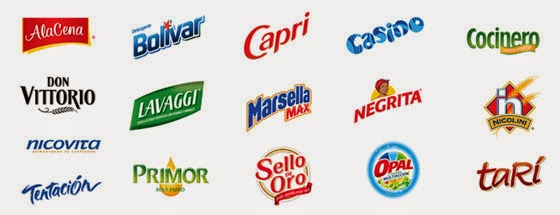
\includegraphics[width=0.9\textwidth]{productos_marcas.jpg}
    \caption{Marca de algunos productos de Alicop}
\end{figure}

\begin{figure}[!ht]
    \centering
    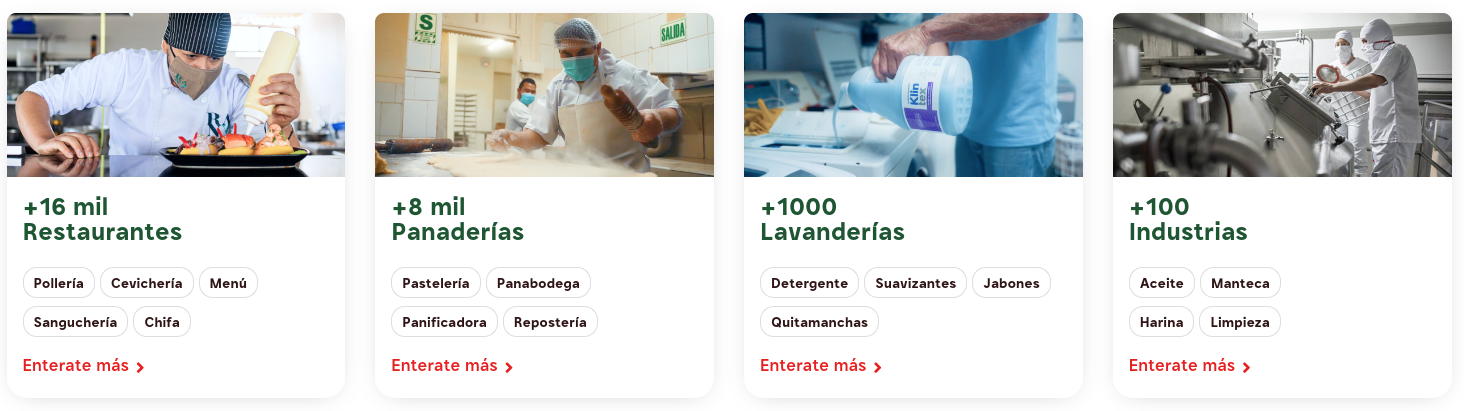
\includegraphics[width=0.95\textwidth]{productos_alicorp_soluciones.png}
    \caption{Captura de la página web Alicop soluciones}
\end{figure}

\begin{figure}[!ht]
    \centering
    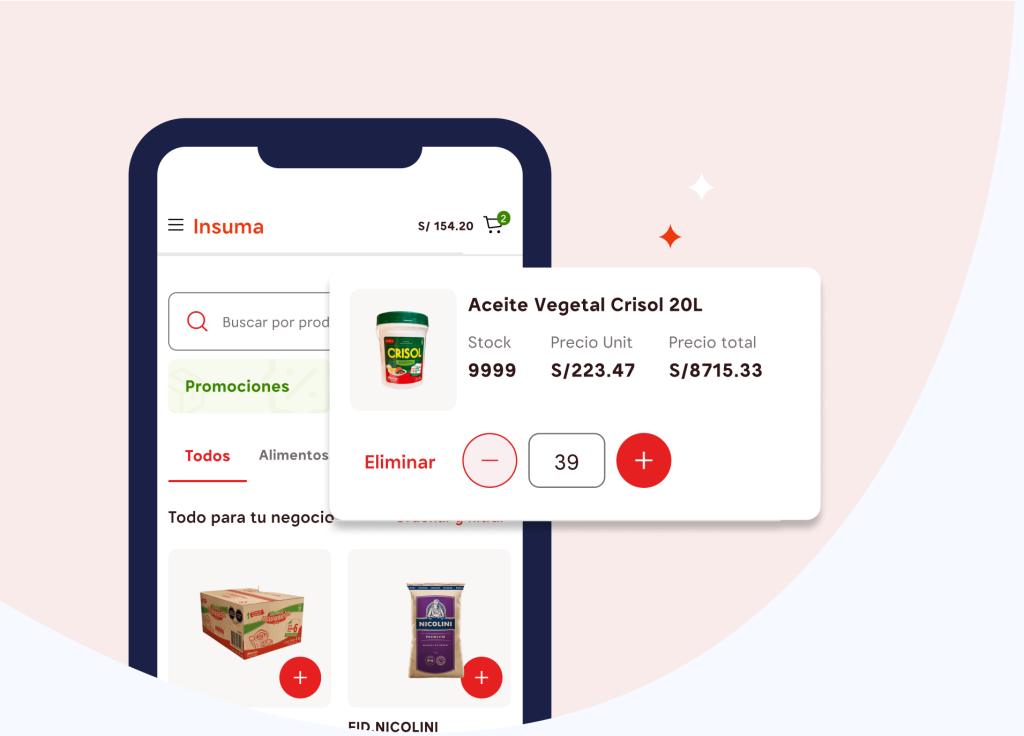
\includegraphics[width=0.95\textwidth]{producto_insuma_app.png}
    \caption{App insuma para la logística entre clientes}
\end{figure}

\begin{figure}[!ht]
    \centering
    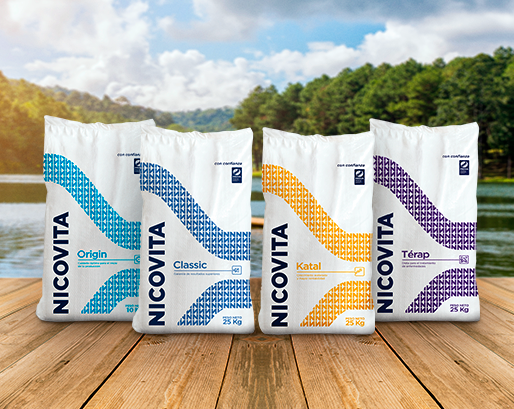
\includegraphics[width=0.7\textwidth]{producto_nicovita.png}
    \caption{Producto nicovita}
\end{figure}

\end{itemize}
